After the discovery of the Higgs boson at the LHC, the first exploration of the couplings of the new particle at Run I and Run II has achieved an overall precision at the level of ten percent. One of the main goals of Higgs studies at the HL-LHC or HE-LHC will be to push the sensitivity to deviations in the Higgs couplings close to the percent level. 

In this section we study the projected precision that would be possible at such high luminosity and high energy extensions of the LHC from a global fit to modifications of the different single-Higgs couplings. Other important goals of the Higgs physics program at the HL/HE-LHC, such as extending/complementing the studies of the total rates with the information from differential distributions, or getting access to the Higgs trilinear coupling, will be covered in other parts of this document. 


In order to study single-Higgs couplings, we introduce a parametrisation, the nonlinear EFT, that transparently connects with the $\kappa$-formalism, but is based on the language of effective field theories (EFTs). 
 We then present a fit to the projected HL/HE-LHC uncertainties both in the $\kappa$-formalism and in the more general nonlinear EFT, discussing the expected sensitivities to deviations on the Higgs couplings at the HL/HE-LHC, and compare with the recent results obtained using current data from \cite{deBlas:2018tjm}. We also translate the results into the EFT formalism relevant for composite Higgs scenarios, discussed in section~\ref{sec9:CHM}.
 

%\subsubsection{Kappa-formalism and the nonlinear EFT}
%\label{sec2:kappavsEFT}
%\wip{This section was moved from the previous subsection and still needs to be polished!}\\

The $\kappa$-formalism was introduced in\cite{LHCHiggsCrossSectionWorkingGroup:2012nn,Heinemeyer:2013tqa} as an interim framework to report on the measurements of the Higgs-boson couplings and characterize the nature of the Higgs boson. The $\kappa_{i}$ are defined as ratios of measured cross sections and decay widths with respect to their SM expectation, {\it i.e.}
\begin{equation}
  \label{eq:kappa.EFT.1}
  \kappa^{2}_{X} = \frac{\sigma(X_i\rightarrow h+X_f)}{\sigma(X_i\rightarrow h+X_f)_{\text{SM}}}, \qquad \kappa^{2}_{Y} = \frac{\Gamma(h\rightarrow Y)}{\Gamma(h\rightarrow Y)_{\text{SM}}},
\end{equation}
so that the SM is recovered for $\kappa_i=1$.
This framework, defined at the level of signal strengths, was appropriate for the observables under study at Run I, which tested deviations in event rates. For Run II and the analyses required at the HL/HE-LHC, differential information is needed and the formalism defined by eq.~\eqref{eq:kappa.EFT.1} has to be extended.
In practice it then becomes more efficient to work directly at the level of Lagrangians. 
Here we will discuss the interpretation of the $\kappa$ factors within the electroweak chiral Lagrangian (EWChL or  HEFT). Within this EFT, the contributions to processes with a single Higgs, in the unitary gauge, are \cite{Buchalla:2015qju,Buchalla:2015wfa,deBlas:2018tjm}
\begin{align}
  \begin{aligned}
    \label{eq:kappa.EFT.2}
    \mathcal{L}_{\text{fit}} &= 2 c_{V} \left(m_{W}^{2}W_{\mu}^{+}W^{-\mu} +\tfrac{1}{2} m^2_Z Z_{\mu}Z^{\mu}\right) \dfrac{h}{v} - \sum_{\psi}c_{\psi} m_{\psi} \bar{\psi} \psi \dfrac{h}{v} \\
 &+ \dfrac{e^{2}}{16\pi^{2}} c_{\gamma} F_{\mu\nu}F^{\mu\nu} \dfrac{h}{v}+ \dfrac{e^{2}}{16\pi^{2}} c_{Z\gamma} Z_{\mu\nu}F^{\mu\nu} \dfrac{h}{v}+\dfrac{g_{s}^{2}}{16\pi^{2}} c_{g}\mathrm{tr}\big[ G_{\mu\nu}G^{\mu\nu}\big]\dfrac{h}{v},
  \end{aligned}
\end{align}
where $m_{i}$ is the mass of particle $i$, $\psi \in \{t, b, c, \tau, \mu\}$, and the $c_{i}$ describe the modifications of the Higgs couplings.
The previous Lagrangian differs from a naive rescaling of Higgs couplings, even though superficially it might seem to be equivalent. In particular, the Standard Model is consistently recovered in eq.~\eqref{eq:kappa.EFT.2} for
\begin{equation}
  \label{eq:kappa.EFT.3}
    c_{i}^{\text{SM}} = \begin{cases} 1 & \text{for } i = V, t, b, c, \tau, \mu\\ 0 & \text{for } i = g, \gamma, Z\gamma. \end{cases}
\end{equation} 
This Lagrangian, taken in isolation, leads to a theory with a parametrically low cutoff: it has therefore to be thought as part of a bigger EFT: the EWChL\cite{Dobado:1989ax,Dobado:1989ue,Dobado:1990zh,Dobado:1990jy,Espriu:1991vm,Herrero:1993nc,Herrero:1994iu,Feruglio:1992wf,Bagger:1993zf,Koulovassilopoulos:1993pw,Burgess:1999ha,Wang:2006im,Grinstein:2007iv,Azatov:2012bz,Alonso:2012px,Buchalla:2012qq,Buchalla:2013rka,Buchalla:2013eza}. This is a bottom-up EFT, constructed with the particle content and symmetries of the SM. These are the same requirements adopted in the construction of the SMEFT. The main difference between both EFTs concerns the Higgs field. In the EWChL, the Higgs boson, $h$, is included as a scalar singlet, with couplings unrelated to the ones of the Goldstone bosons of EWSB. 
Therefore, $h$ is not necessarily part of an SU(2) doublet and consequently (contrary to the SMEFT) the leading-order Lagrangian is already an EFT, leading potentially to $O(1)$ effects in the $\kappa$s and to a potentially low cutoff.
Further details and explanations  are discussed in \cite{Guo:2015isa,Buchalla:2017jlu,Alonso:2017tdy,Buchalla:2013rka,Buchalla:2013eza,Buchalla:2015wfa,Buchalla:2016sop}.

Focussing on the leading effects in single-Higgs processes only, the full EWChL reduces to eq.~\eqref{eq:kappa.EFT.2} which, if needed,  can be extended to describe other processes:   double-Higgs production from gluon fusion, for instance, would require three more operators, corresponding to the interactions $h^{3},\bar{t}th^{2},ggh^{2}$~\cite{Grober:2015cwa,deFlorian:2016spz,Kim:2018uty,Buchalla:2018yce} (see section~\ref{sec:EWChL.double.h}). Since the observed processes are mediated by both tree level and one-loop amplitudes at the first non-vanishing order, operators of leading order in the EFT (first line of eq.~\eqref{eq:kappa.EFT.2}) and next-to-leading order in the EFT (second line of eq.~\eqref{eq:kappa.EFT.2}) have to be included\cite{Buchalla:2015wfa}. Corrections beyond the leading ones, both strong and electroweak, can also be incorporated to arbitrary order in the description of Higgs processes. These corrections involve additional operators, not present in eq.~\eqref{eq:kappa.EFT.2}, but contained in the EWChL.
 
As stated above, the couplings in eq.~\eqref{eq:kappa.EFT.2} can receive a priori large contributions and have to be considered as $\mathcal{O}(1)$ numbers. This is the expectation if new physics contains strongly-coupled new interactions at the electroweak scale. In other scenarios of compositeness, new-physics interactions  can be associated with a larger scale $f$ and progressively decoupled from the SM: it is therefore useful to understand the Wilson coefficients in eq.~\eqref{eq:kappa.EFT.2} as functions of the parameter $\xi = v^{2}/f^{2}$. The scale $f$ could correspond, for example, to the scale of global symmetry breaking in composite Higgs models (see the discussion in sec.~\ref{sec9:CHM}). The SM is then recovered for $\xi=0$. For $\xi\ll 1$, one can perform an expansion in $\xi$ on top of the loop expansion in the EWChL. This yields a double expansion in $\xi$ and $1/16\pi^{2}$ \cite{Buchalla:2014eca}, in the spirit of the strongly-interacting light Higgs (SILH) \cite{Giudice:2007fh}. The expected size of the Wilson coefficients is then
\begin{equation}
  \label{eq:kappa.EFT.4}
    c_{i} =  c_{i}^{\text{SM}} + \mathcal{O}(\xi).
\end{equation}
The mapping of the Wilson coefficients $c_{i}$ to the $\kappa_{i}$ parameters is done using the relations of the signal strengths computed from the Lagrangian in eq.~\eqref{eq:kappa.EFT.2}. The necessary formulas can be found in \cite{Buchalla:2015qju,deBlas:2018tjm}. These relations can be written as
%
\begin{equation}
\label{eq:kappa.EFT.5}
  \kappa_{i} =  |f_i(c_{j})| \equiv \frac{|{\cal A}_i(c_{j})|}{|{\cal A}_i(c_{j}^{\text{SM}})|}, 
\end{equation}
%
where ${\cal A}$ is the corresponding transition amplitude of each process (the absolute value on the right hand side is necessary, as the loop functions of the light fermions ($b,\tau,\mu,\dots$) for the $\kappa_{\gamma}$ and $\kappa_{g}$ are complex)
We can  obtain an approximate inverse of eq.~\eqref{eq:kappa.EFT.5}, to connect both formalisms in the opposite direction, by assuming that all the imaginary parts are negligible.\footnote{This is a good approximation for some of the coefficients in $f_i(c_{j})$, for example for the coefficient of $c_{t}$, or as long as  the Wilson coefficients stay relatively close to the SM value. This is not the case for the coefficients of the light fermion loops, where real and imaginary parts are of similar size.}
With the assumption of vanishing imaginary parts, eq.~\eqref{eq:kappa.EFT.5} becomes
\begin{equation}
  \label{eq:kappa.EFT.6}
  \begin{pmatrix}
    \kappa_{V}\\
    \kappa_{t}\\
    \kappa_{b}\\
    \kappa_{\ell}\\
    \kappa_{g}\\
    \kappa_{\gamma}
  \end{pmatrix}
  = 
  \begin{pmatrix}
    1 & 0 & 0 & 0 & 0 & 0 \\
    0 & 1 & 0 & 0 & 0 & 0 \\
    0 & 0 & 1 & 0 & 0 & 0 \\
    0 & 0 & 0 & 1 & 0 & 0 \\
    0 & 1.055 & -0.055 & 0 & 1.3891 & 0 \\
    1.2611 & -0.2683 & 0.0036 & 0.0036 & 0 & -0.3039 \\
  \end{pmatrix}
  \cdot
  \begin{pmatrix}
    c_{V}\\
    c_{t}\\
    c_{b}\\
    c_{\tau}\\
    c_{g}\\
    c_{\gamma}
  \end{pmatrix}.
\end{equation}
%
These numbers also include the leading QCD corrections of the $h\to \gamma\gamma$ and $gg\to h$ amplitude. An explicit comparison of this approximation and the full formulas shows only negligible numerical differences. The inverse of eq.~\eqref{eq:kappa.EFT.6} is
\begin{equation}
  \label{eq:kappa.EFT.7}
  \begin{pmatrix}
    c_{V}\\
    c_{t}\\
    c_{b}\\
    c_{\tau}\\
    c_{g}\\
    c_{\gamma}
  \end{pmatrix}
  = 
  \begin{pmatrix}
    1 & 0 & 0 & 0 & 0 & 0 \\
    0 & 1 & 0 & 0 & 0 & 0 \\
    0 & 0 & 1 & 0 & 0 & 0 \\
    0 & 0 & 0 & 1 & 0 & 0 \\
    0 & -0.76 & 0.04 & 0 & 0.72 & 0 \\
    4.15 & -0.88 & 0.012 & 0.012 & 0 & -3.29 \\
  \end{pmatrix}
  \cdot
  \begin{pmatrix}
    \kappa_{V}\\
    \kappa_{t}\\
    \kappa_{b}\\
    \kappa_{\ell}\\
    \kappa_{g}\\
    \kappa_{\gamma}
  \end{pmatrix}.
\end{equation}
%
With these relations one can translate the results of a $\kappa_i$ fit into the EWChL~formalism and vice-versa. \\

\noindent
{\bf Fit to HL/HE-LHC Higgs precision data.}
The fits presented in what follows have been performed using the {\tt HEPfit} package~\cite{hepfit,hepfitsite}, and following a statistical Bayesian approach.  
 The prior for the different model parameters both in the EFT and in the $\kappa$ framework are taken as flat, centered around the SM solution, and restricting the ranges to avoid other solutions present due to the parametrization invariances of the different formalisms.
Since no sensitivity to the $H\to c\bar{c}$ channel at the HL/HE-LHC has been reported yet we fix the corresponding parameters controlling the $Hc\bar c$ interactions to their SM values ($c_c,\kappa_c=1$).~\footnote{See ~\cite{deBlas:2018tjm} for a discussion of the multiplicities of the different solutions in the fit as well as the effect of letting the charm coupling float in the fits in absence of a significant direct constraint.}

To assess the sensitivity to deviations from the SM, we assume the future measurements are SM-like and include them in the likelihood of the fit assuming Gaussian distributions with standard deviations given by the corresponding experimental uncertainty. 

The analysis of current constraints has been taken directly from~\cite{deBlas:2018tjm}, which is based on the experimental data from~\cite{Aaltonen:2013ipa,Abazov:2013gmz,Chatrchyan:2013iaa,Chatrchyan:2013vaa,Chatrchyan:2013zna,Aad:2014eha,Aad:2014eva,Aad:2014xzb,ATLAS:2014aga,Chatrchyan:2014nva,Khachatryan:2014ira,Khachatryan:2014jba,Khachatryan:2014qaa,Aad:2015gba,Aad:2015gra,Aad:2015ona,Aad:2015vsa,ATLAS:2016gld,CMS:2016mmc,Khachatryan:2016vau,Aaboud:2017jvq,Aaboud:2017ojs,Aaboud:2017rss,Aaboud:2017uhw,Aaboud:2017vzb,Aaboud:2017xsd,CMS:2017rli,CMS-PAS-HIG-17-007,CMS-PAS-HIG-17-019,Sirunyan:2017elk,Sirunyan:2017exp,Sirunyan:2017khh,Aaboud:2018xdt,ATLAS-CONF-2018-004,Sirunyan:2018egh,Sirunyan:2018mvw,Sirunyan:2018shy,Sirunyan:2018ygk}. 
For the HL-LHC fits we use the corresponding ATLAS and CMS projections presented in this document. (See section~\ref{sec2:expan} and section~\ref{sec2:exp_combination}.)  For the systematics and theory uncertainties we use the 2 scenarios presented in section~\ref{sec:HiggsExtrapAss}: S1, for which the systematics are kept as in current values, and S2, where experimental systematics are reduced with the luminosity and theory errors are reduced.
%
The correlations between the ATLAS and CMS sets of inputs were not available for these fits, and are therefore ignored. We note that the absence of that information can result, in some cases, in somewhat optimistic bounds. This is particularly the case for those couplings whose uncertainty is dominated by theoretical errors (e.g. $\kappa_t$).

%
Finally, we follow the ATLAS and CMS guidelines to estimate the HE-LHC uncertainties for the different signal strengths.  
Starting from the HL-LHC S2 projections we define the {\it Base} HE-LHC scenario by scaling the statistical uncertainties according to the changes in the production cross section going from 14 TeV to 27 TeV, as well as the different luminosities (3 ab$^{-1}$ for the HL-LHC and 15 ab$^{-1}$ in the HE-LHC):
%
\begin{equation}
\delta_{\mathrm{stat}} \mu_{\mbox{\tiny HE-LHC}} = \sqrt{\frac{\sigma_{pp\to H}^{\mathrm{14 TeV}}\times 3~\!\mathrm{ab}^{-1}}{\sigma_{pp\to H}^{\mathrm{27 TeV}}\times 15~\! \mathrm{ab}^{-1}}} \delta_{\mathrm{stat}} \mu_{\mbox{\tiny HL-LHC}} .
\end{equation}
%
Other experimental and theory uncertainties are kept as in the HL-LHC S2 case. 
To compare the results with those that would be possible in a scenario where better understanding of theory errors or systematics is achieved, it was suggested to use a more optimistic scenario where such uncertainties are further reduced by a factor of 2. We also include this optimistic scenario in our fits, and we denote it by {\it ``Opt.''}. One should note, however, that such a scenario does not come from a systematic extrapolation of the possible reduction of uncertainties. It is only an educated guess for illustration purposes.
\vspace{1cm}
 

In Table~\ref{tab:projection.ci} we show the results of the fit for the different scenarios discussed above for the EWChL. The numbers for the HL-LHC and the HE-LHC are reported independently (i.e. the HE-LHC does not includes the HL-LHC results on the Higgs couplings). %No form of correlation between the HL-LHC and HE-LHC estimates is included, and therefore the 
%results may be too optimistic. 
These results are also shown in Figure~\ref{fig:projection.ci}. 
The analogous results for the fit using the $\kappa$ formalism are presented in Table~\ref{fig:projection.kappai} and Figure~\ref{fig:projection.kappai}. In order to put both approaches on an equal theoretical footing, in the $\kappa$ fit we assumed custodial symmetry as well as the absence of extra exotic decays of the Higgs.  As expected from the discussion above, the results show an excellent agreement between the $c_i$ and $\kappa_i$ fits for most of the parameters. The exceptions are the parameters entering in loop-induced processes, $c_{g,\gamma}$ and $\kappa_{g,\gamma}$, whose interpretation differs in the two formalisms. In particular, the interplay between $c_{\gamma}$ and the couplings modifying the SM loops results in a significant difference between the $c_\gamma$ result and the one for $\kappa_\gamma$.

Focussing our attention on the HL-LHC results, we observe that, even in the conservative S1 scenario, knowledge of the different EFT parameters, $c_i$, and Higgs-couplings modifiers, $\kappa_i$, will improve by at least a factor of 2-3 with respect to current experimental limits. The improvement is more marked for channels that benefit from very high statistics, such as $H\to \mu^+ \mu^-$, with a precision $\sim 7$ times better than in the current fit. Further progress is expected at the HE-LHC where, for instance, we foresee
$1\%$ level determinations for the Higgs couplings to vector bosons and $\tau$ leptons.
As one can see by comparing the HL-LHC S2 and HE-LHC Base scenarios, the precision of the interactions associated with the main Higgs couplings 
will be controlled, to a large extent, by systematic and theory errors. 

One must be careful with the interpretation of these results, though. These projections implicitly assume that departures from the SM appear only as modifications in the Higgs couplings or, in other words, that any other interaction entering the relevant Higgs processes is exactly SM-like. However, at the level of precision we observe in the results, close to the $1\%$, this may not be a justified assumption given current bounds on other electroweak interactions that could modify, e.g.~VBF or VH associated production. This comment applies even more to the HE-LHC uncertainties obtained assuming the reduced theory and systematic uncertainties which, in particular, predict a subpercent precision for the Higgs coupling to vector bosons. We believe this to be too aggressive. A more realistic assessment of the HE-LHC uncertainties would require an equally realistic study of the experimental precision at that machine, as well as the results of a full global fit combining Higgs data with other relevant observables of the EW sector. We refer to section~\ref{sec8} for more details in this regard.

\begin{table}[ht!]
\begin{center}
\caption{Comparison of the current and HL/HE-LHC 68\% probability sensitivities to the $c_{i}$ coefficients, as shown in Figure~\ref{fig:projection.ci}.}\label{tab:projection.ci}
\begin{tabular}{  c c c c c c }
  \hline\hline
  & Current limits~\cite{deBlas:2018tjm}  & HL-LHC S1 & HL-LHC S2 & HE-LHC (Base)&HE-LHC (Opt.) \\
  \hline
   $c_{V}$&$1.01\pm0.06$ &$\pm 0.017$&$\pm 0.011$&$\pm 0.009$&$\pm 0.005$\\
  $c_{t}$&$1.04^{+0.09}_{-0.1}$&$\pm 0.040$&$\pm 0.025$&$\pm 0.020$&$\pm 0.010$\\
  $c_{b}$&$0.95\pm0.13$ &$\pm 0.042$&$\pm 0.028$&$\pm 0.023$&$\pm 0.012$ \\
  $c_{\tau}$&$1.02\pm 0.1$ &$\pm 0.023$&$\pm 0.017$& $\pm 0.012$&$\pm 0.007$\\
  $c_{\mu}$&$0.58^{+0.4}_{-0.38} $ &$\pm 0.056$&$\pm 0.044$& $\pm 0.020$&$\pm 0.014$\\
  $c_{g}$&$-0.01^{+0.08}_{-0.07} $ &$\pm 0.032$&$\pm 0.020$& $\pm 0.016$&$\pm 0.008$\\
  $c_{\gamma}$ &$0.05\pm0.2 $&$\pm 0.066$&$\pm 0.045$&$\pm 0.033$&$\pm 0.019$\\
  %$c_{Z\gamma}$ &$-$&$\pm $&$\pm $&$\pm $&$\pm $\\
\hline\hline
\end{tabular}
\end{center}
\end{table}
%
\begin{figure}[ht]
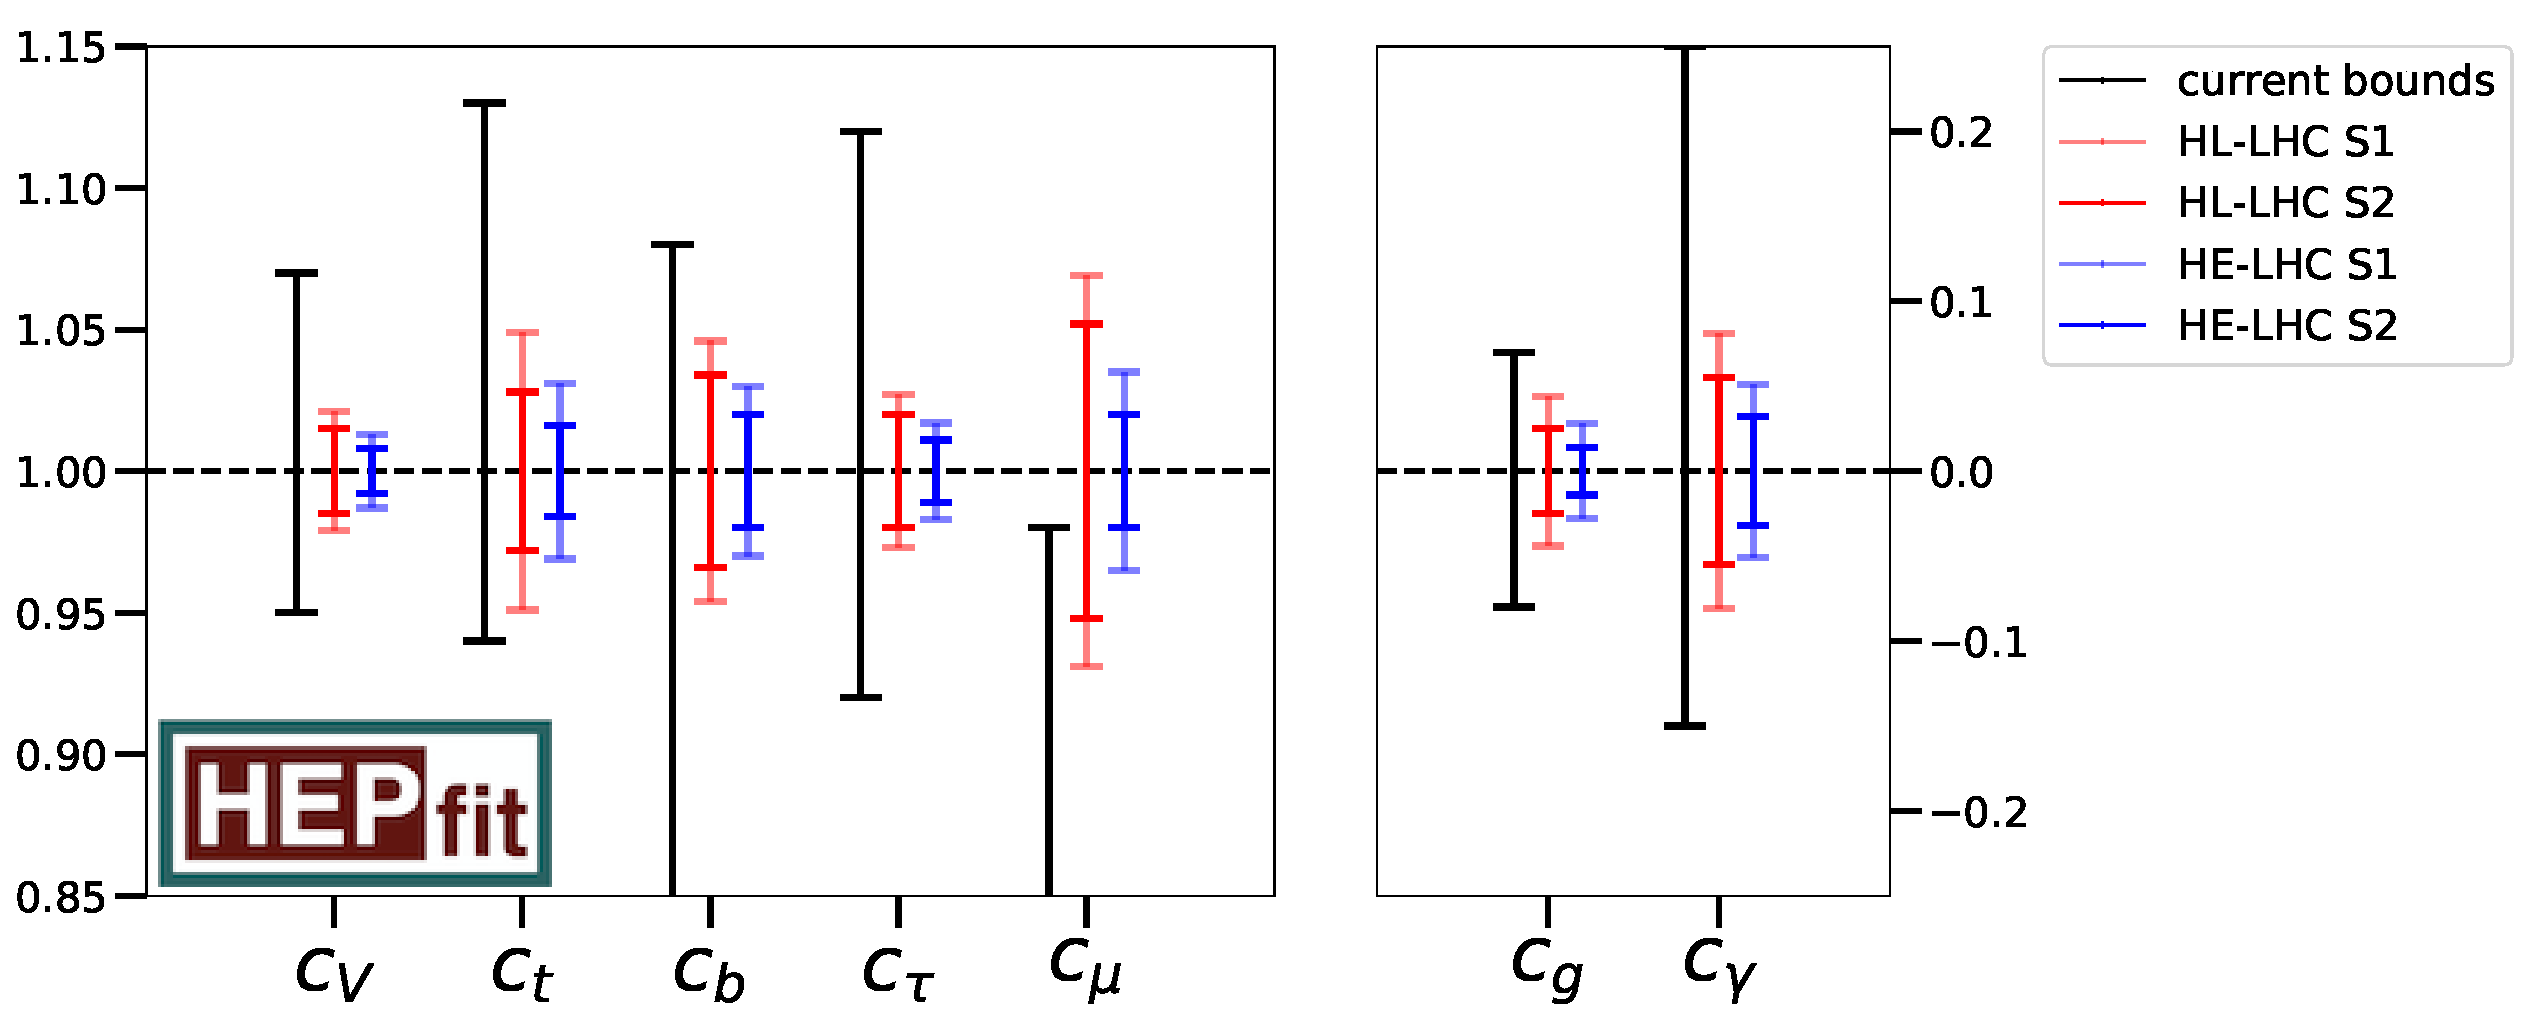
\includegraphics[width=\textwidth]{\main/section2/plots/fit_summary_ci.pdf}
\caption{Current and HL/HE-LHC constraints on $c_{i}$. The left line of each coupling is the current bound, from Ref.~\cite{deBlas:2018tjm}. The central line is the projection to the HL-LHC, with the S1 scenario in light red and S2 in dark red. The right line is the projection to HE-LHC, with the base scenario in light blue and the optimistic one in dark blue.}\label{fig:projection.ci}
\end{figure}

\begin{table}[ht!]
\begin{center}
\caption{Comparison of the current and HL/HE-LHC 68\% probability sensitivities to the SM Higgs-coupling modifiers $\kappa_{i}$, as shown in Figure~\ref{fig:projection.kappai}.}\label{tab:projection.kappai}
\begin{tabular}{ c c c c c c }
  \hline\hline
  & Current limits~\cite{deBlas:2018tjm}  & HL-LHC S1 & HL-LHC S2 & HE-LHC (Base)&HE-LHC (Opt.) \\
  \hline
   $\kappa_{V}$&$1.01\pm0.06$ &$\pm 0.017$&$\pm 0.011$&$\pm 0.009$&$\pm 0.005$\\
  $\kappa_{t}$&$1.04^{+0.09}_{-0.1}$&$\pm 0.040$&$\pm 0.025$&$\pm 0.020$&$\pm 0.010$\\
  $\kappa_{b}$&$0.94\pm 0.13$ &$\pm 0.042$&$\pm 0.028$&$\pm 0.023$&$\pm 0.012$ \\
  $\kappa_{\tau}$&$1.0\pm 0.1$ &$\pm 0.023$&$\pm 0.017$& $\pm 0.012$&$\pm 0.007$\\
  $\kappa_{\mu}$&$0.58^{+0.4}_{-0.38} $ &$\pm 0.056$&$\pm 0.044$& $\pm 0.020$&$\pm 0.014$\\
  $\kappa_{g}$&$1.02^{+0.08}_{-0.07} $ &$\pm 0.027$&$\pm 0.018$& $\pm 0.015$&$\pm 0.008$\\
  $\kappa_{\gamma}$ &$0.97\pm 0.07 $&$\pm 0.023$&$\pm 0.016$&$\pm 0.012$&$\pm 0.007$\\
 % $\kappa_{Z\gamma}$ &$-$&$\pm $&$\pm $&$\pm $&$\pm $\\
\hline\hline
\end{tabular}
\end{center}
\end{table}
%
\begin{figure}[ht]
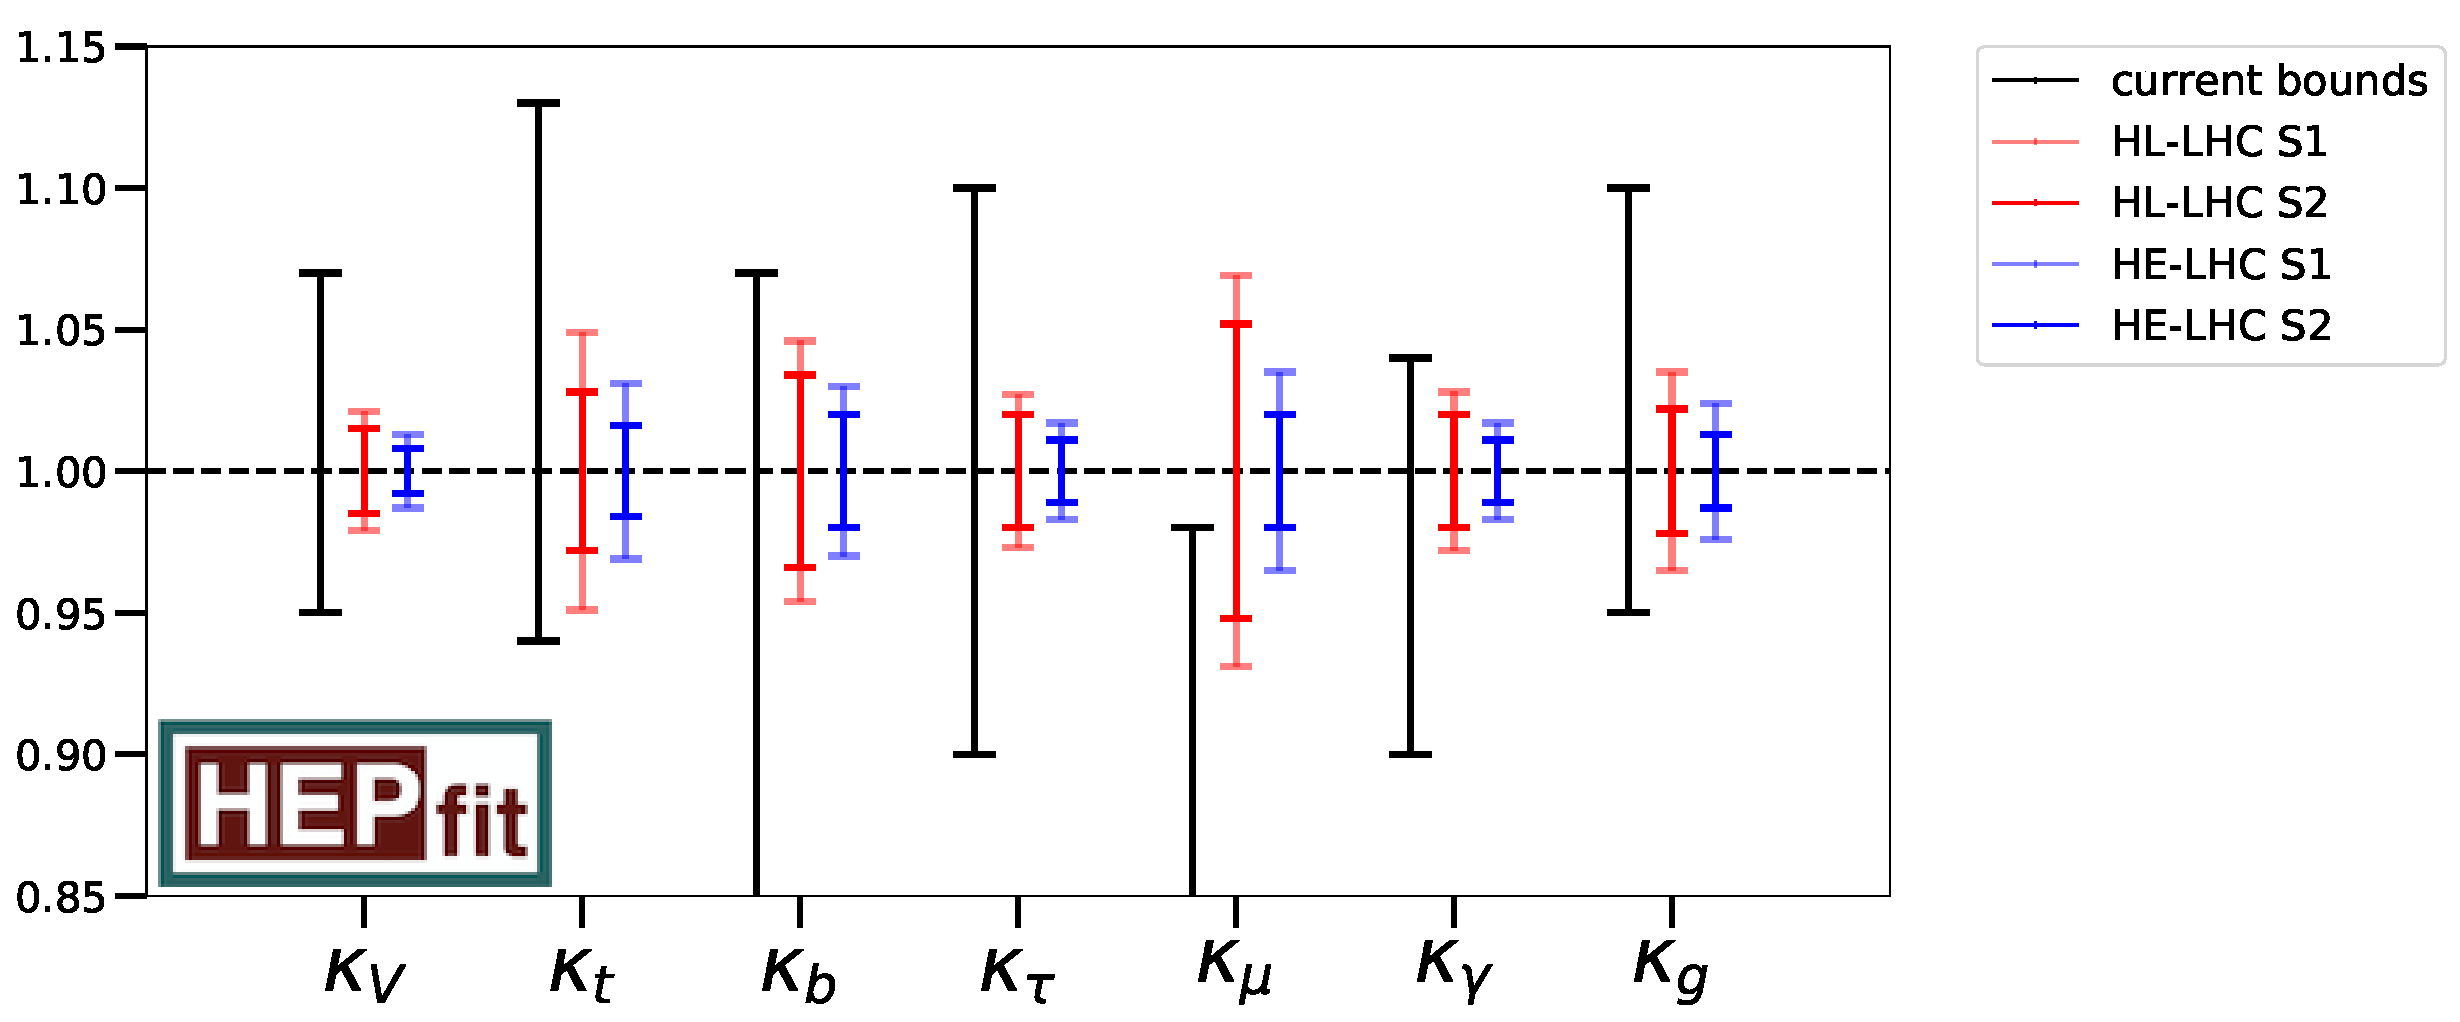
\includegraphics[width=\textwidth]{\main/section2/plots/fit_summary_kappai.pdf}
\caption{Current and future constraints on $\kappa_{i}$. The left line of each $\kappa$ is the current bound, from Ref.~\cite{deBlas:2018tjm}. The central line is the projection to the HL-LHC, with the S1 scenario in light red and S2 in dark red. The right line is the projection to HE-LHC, with the base scenario in light blue and the optimistic one in dark blue.}\label{fig:projection.kappai}
\end{figure}
